\begin{scanpage}{0188}{170}
\begin{center}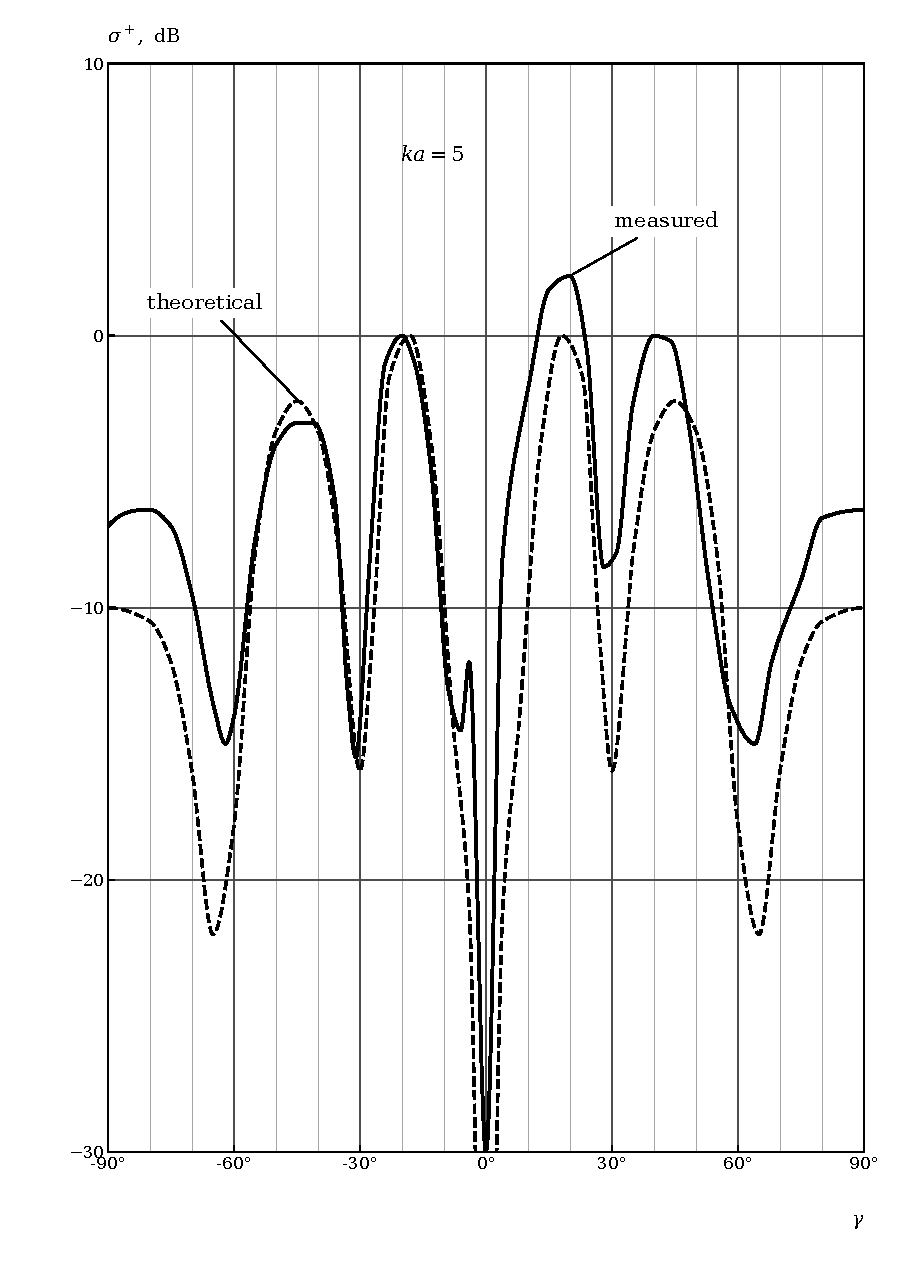
\includegraphics[width=.58\linewidth]{images/recreated/c-0188-fig71.pdf}\par
Figure 71. Diagram of the radiation from the nonuniform part of the current flowing on a disk.
\end{center}
approximation character of the computational equations. The value $\gamma=90^\circ$ corresponds to the direction along the disk's surface, and the value $\gamma=0^\circ$---to the direction normal to the disk.
\sectiontitle{27}{Reflected Wave Depolarization}
Let us again return to the problem of scattering of an electromagnetic wave by an arbitrary metal body. The relative position of the source Q, of a surface element of the irradiated body, and of the coordinate system is shown in Figure 69. Let us recall that the
\end{scanpage}
